\documentclass{article}

\usepackage[left=1in, right=1in, top=1in, bottom=1in]{geometry}

\usepackage{setspace}
\usepackage{fancyhdr}
\usepackage{hyperref}
\usepackage{amsthm}
\usepackage{amssymb}
\usepackage{multirow}
\usepackage{enumitem}
\usepackage{graphicx}
\usepackage{makecell}
\usepackage{booktabs}
\usepackage{titlesec}
\usepackage{amsmath}
\usepackage{pdfpages}

\setcounter{secnumdepth}{4}

\hypersetup{
    colorlinks=true,     
    urlcolor=magenta
}

\renewcommand{\qedsymbol}{\rule{0.7em}{0.7em}}

\newlength\tindent
\setlength{\tindent}{\parindent}
\setlength{\parindent}{0pt}
\renewcommand{\indent}{\hspace*{\tindent}}
\setlength{\parskip}{0em}

\newenvironment{blockquote}{%
  \par%
  \vskip1em
  \leftskip=2em\rightskip=2em%
  \noindent\ignorespaces}{%
  \par\vskip1em}

\newenvironment{blockquote2}{%
	\par%
	\vskip1em
	\leftskip=4em\rightskip=4em%
	\noindent\ignorespaces}{%
	\par\vskip1em}

\pagestyle{fancy}
\fancyhf{}
\fancyhead[LO]{STA5176}
\fancyhead[RO]{Kyle Ligon}
\fancyfoot[LO]{Chapter 6}
\fancyfoot[RO]{\thepage}
 
\renewcommand{\headrulewidth}{0.5pt}
\renewcommand{\footrulewidth}{0.5pt}

\begin{document}
\section*{Chapter 6 Homework}
\subsection*{Due 2-18-2018}
\subsubsection*{Problem 6.13}
\subsubsection*{a) Complete a Hypothesis Test for $\mu_1$-$\mu_2$; $\alpha$ = 0.05}
Hypotheses:
\begin{blockquote}

	$H_0: \mu_{Female} - \mu_{Male} = 0$

	$H_{A}: \mu_{Female} - \mu_{Male} \neq 0$
\end{blockquote}

Assumptions:
\begin{blockquote}
	1) Independent Samples.  

	2) Equal Variances.  ($\sigma_F^{2} = 1.4136,  \sigma_M^{2} = 1.0077$)
\end{blockquote}

Test Statistic: 
\begin{eqnarray}
	t_0 = \frac{\bar{y_{F}}-\bar{y_{M}}-D_0}{s_p\sqrt{\frac{1}{n_{F}}+\frac{1}{n_{M}}}} \nonumber \\
	t_0 = \frac{(8.5333 - 9.6833)-0}{1.0719\sqrt{0.0417+0.0278}} \nonumber \\
	t_0 = \frac{-1.15}{0.2826} \nonumber \\
	t_0 = -4.0708 \nonumber
\end{eqnarray}
Rejection Region:
\begin{blockquote}
$|t_0| \geq t_{\frac{\alpha}{2}, 58};  t_{\frac{\alpha}{2}, 58} = 2.0017$

Thus, $|-4.0708| = 4.0708 \geq 2.0017$
\end{blockquote}

P-Value
\begin{blockquote}
The p-value on a t-score of -4.0708 = $7.1822$x$10^{-5}.$   

Therefore, our p-value is less than our $\alpha$ of 0.025.  
\end{blockquote}

Conclusion/Interpretation:
\begin{blockquote}
Since the absolute value of our t-score is greater than our Rejection Boundary, there is sufficient evidence to reject our Null Hypothesis of $\mu_{F}-\mu_{M} = 0$.  There is evidence to suggest that the two mean pays between the Male and Female group are different.  
\end{blockquote}

\subsubsection*{b) Complete a 95\% C.I. for $\mu_{F} - \mu_{M}$}
Assumptions:
\begin{blockquote}
1) We are still under the assumption that these two groups were chosen independently.

2) We are also under the assumption that the Variances are equal and holding from the last section.  
\end{blockquote}
Confidence Interval Equation:
\begin{eqnarray}
	C.I. = \bar{y_F}-\bar{y_M} \pm t_{\frac{\alpha}{2}, df}\left(\frac{s_F^{2}}{\sqrt{n_F}} + \frac{s_M^{2}}{\sqrt{n_M}}\right) \nonumber \\
	C.I. =  (8.5333 - 9.6833) \pm 2.0017\left(\frac{1.4136}{4.8990}+\frac{1.0077}{6}\right) \nonumber \\
	C.I. = -1.15 \pm 2.0017(0.4565) \nonumber \\ 
	C.I. = -1.15 \pm 0.9138 \nonumber \\
	C.I \approx (-2.0638, -0.2362)  \nonumber 
\end{eqnarray}

Conclusion/Interpretation:
\begin{blockquote}
Since 0 is not in our confidence interval, we can conclude we have strong enough evidence to suggest that the population mean pays between men and women at this firm are different.  (This supports the hypothesis test we did in part a).)  
\end{blockquote}

\subsubsection*{Problem 6.15}
\subsubsection*{ Random samples of size $n_1$ = 8 and $n_2$ = 8 were selected from populations A and B, respectively.}
\subsubsection*{a) Test for a difference in the medians of the two populations using an $\alpha$ = 0.05 Wilcoxon Rank Sum Test.}

Hypotheses:
\begin{blockquote}
	$H_0: M_A = M_B$

	$H_A: M_A \neq M_B$
\end{blockquote}

Assumptions:
\begin{blockquote}
1) Independent Random Samples

2) Population distributions are the same shape, except one is shifted from the other
\end{blockquote}

Test Statistic:
\begin{blockquote}
With both $n_A$ and $n_B = 8$, we will perform the Wilcoxon Rank Sum Test.  In order to arrive at our test statistic, we must rank the values of each group concurrently.  Then, we will sum Group A to check to see if it's greater than our Rejection Boundary.  We handle ties in the ranking by averaging their respective ranks together.  (e.g. both 4.4's will have a rank of 6.5 because they're in the $6^{th}$ and $7^{th}$ ranks.) See Table 1 for the rankings.  
\end{blockquote} 

\begin{table}[ht]
\caption{Wilcoxon Rank Sum Test for Population A and Population B}
\centering
\begin{tabular}{c c c}
\hline\hline
Value & Rank & Group \\ [0.5ex] 
\hline
3.5 & 1 & B  \\
3.7 & 2 & B  \\
3.8 & 3 & B  \\
3.9 & 4 & B  \\
4.3 & 5 & A  \\ 
4.4 & 6.5 & B  \\ 
4.4 & 6.5 & B  \\
4.6 & 8 & A  \\
4.7 & 9.5 & A  \\
4.7 & 9.5 & B  \\
5.1 & 11 & A  \\  
5.2 & 12 & B  \\
5.3 & 13.5 & A  \\
5.3 & 13.5 & A  \\ 
5.4 & 15 & A  \\ 
5.8 & 16 & A  \\ [1ex]
\hline
\end{tabular}
\label{table:nonlin}
\end{table}
Calculation:
\begin{blockquote}
$T_0 = \sum\limits_{i = 1}^n r $, where r is the ranks of the values in the 1st Population (Group A in our case) \\
$T_0 = 91.5$
\end{blockquote}

Rejection Region:
\begin{blockquote}
We need both the Upper and Lower bounds of this Rejection Boundaries.  For a Wilcoxon Rank Sum two tail test with $\alpha$ = 0.05 and both sample sizes being 8, $T_L = 49$ and $T_U = 87.$  Since our $T_0 = 91.5 \ge 87 = T_U$, we have enough to make a conclusion.  
\end{blockquote}

P-Value:
\begin{blockquote}
Due to having ties, a true, exact p-value cannot be computed.  However, R's wilcox.test function yields an approximate p-value of 0.01549.  
\end{blockquote}
Conclusion:
\begin{blockquote}
Since our $T_0 \ge T_U$, we have enough statistical evidence to reject the Null Hypothesis that $M_A = M_B$.  There is extreme enough data to indicate that $M_A \neq M_B$.  Our approximated p-value of 0.0149 doubled equals 0.0298.  This p-value backs our above conclusion up since it is less than our $\alpha$ of 0.05.  
\end{blockquote}

\subsubsection*{Problem 6.28}
\subsubsection*{a) Is there significant evidence that the mean SENS value decreased after the patient received antihypertensive treatment?}
Hypotheses:
\begin{blockquote}
\indent In this test, $\mu_1 = \mu_{Before}$ and $\mu_2 = \mu_{After}$.  Therefore, if we want to check if the mean SENS value decreased, our $H_1$ should be $\mu_B-\mu_A \ge 0$.  \\

	$H_0: \mu_B - \mu_A \leq 0$
	
	$H_A: \mu_B - \mu_A > 0$
\end{blockquote}

Assumptions:
\begin{blockquote}
	1) Sampling distributions of $d_{i}'s$ are normally distributed.
	
	2) $d_{i}'s$ are independent.  
\end{blockquote}

Test Statistic:
\begin{blockquote}
With there being a Before and After treatment for 10 patients, we will use the T-test for Paired Data.  In order to begin, we must find the differences for each pair of data.  
\end{blockquote}

\pagebreak

\begin{table}[ht]
\caption{Table for Paired Data to be used in T-test}
\centering
\begin{tabular}{c c c}
\hline\hline
Before & After & Difference \\ [0.5ex] 
\hline
22.86 & 6.11 & 16.75   \\
7.74 & -4.02 & 11.76 \\
15.49 & 8.04 & 7.45  \\
9.97 & 3.29 & 6.68  \\
1.44 & -0.77 & 2.21  \\ 
9.39 & 6.99 & 2.4  \\ 
11.40 & 10.19 & 1.21  \\
1.86 & 2.09 & -0.23  \\
-6.71 & 11.40 & -18.11 \\
6.42 & 10.70 & -4.28 \\ [1ex]
\hline
\end{tabular}
\label{table:nonlin}
\end{table}

\begin{blockquote}
With the differences being found, we must now find the mean of the differences, standard deviations of differences, and number of those paired points.  
\\
$\bar{d} $ = 2.584 \\
$s_d $ = 9.4907 \\
$n_d $ = 10


\begin{eqnarray}
	t_0 = \frac{2.584-0}{\frac{9.4907}{\sqrt{10}}} \nonumber \\
	t_0 = \frac{2.584}{2.8460} \nonumber \\
	t_0 = 0.9079 \nonumber \\
\end{eqnarray}
\end{blockquote}

Rejection Region:
\begin{blockquote}
	With an identified test statistic, we need to find the boundary on our Rejection Region.  With an $\alpha$ of 0.05 and degrees of freedom of 9, our rejection region is at t = 0.9079.  Thus, if our test statistic is greater than 1.833, we'll reject the Null Hypothesis that the SENS value hasn't decreased with the treatment.  
\end{blockquote}

P-value:
\begin{blockquote}
To get the p-value, we check the pt function in R for a test statistic of 0.9079 for 9 degrees of freedom.  The p-value of t = 0.9079 for 9 degrees of freedom is 0.1938.  
\end{blockquote}

Conclusion:
\begin{blockquote}
Since our $t_0 =$ 0.9079 $<$ 1.833 and our p-value = 0.1937 $>$ 0.05, there is not strong evidence that we should reject $\mu_1 - \mu_2 \leq 0$.  Thus, there is not supporting evidence that this treatment decreased SENS value.  
\end{blockquote}

\subsubsection*{b) Estimate the size of the change in the mean SENS value}
\begin{blockquote}
To estimate the size change, we will create a 95\% confidence interval of the mean of the paired data.  
\end{blockquote}

\begin{eqnarray}
C.I. = \bar{d} \pm t_{\frac{\alpha}{2}, df} \left(\frac{s_d}{\sqrt{n}}\right) \nonumber \\
C.I. = 2.584 \pm 2.262\left(2.8460\right) \nonumber \\
C.I. = 2.584 \pm 6.4377 \nonumber \\
C.I. \approx (-3.8537, 9.0217) \nonumber 
\end{eqnarray}

Conclusion/Interpretation:
\begin{blockquote}
We are 95\% confident that the mean difference between the Before and After group is between -3.8537 and 9.0217.  
\end{blockquote}


\subsubsection*{Problem 6.36}
\subsubsection*{Use these data to test the research hypothesis that the distribution of heart rates for the dogs when receiving Benzedrine is shifted to the right of that for the same animals on the placebo.  Use a one-tailed Wilcoxon signed-rank test with $\alpha$ = 0.05}

Hypotheses:
\begin{blockquote}
To begin, $d_{i}'s$ = Placebo - Benzedrine.  Thus, if the Benzedrine group's distribution are shifted to the right, we would expect the $M_{Placebo} - 
M_{Benzedrine} = M < 0$, where M is the hypothesized median of the differences. \\

$H_0: M \geq  0$

$H_1: M < 0$
\end{blockquote}

Assumptions:
\begin{blockquote}
1) Population of $d_i's$ is symmetric about the unknown median M.
\end{blockquote}

Test Statistic:
\begin{blockquote}
With there being a placebo and Benzedrine treatments, we will subtract to find the differences of the two treatments.  \\
\indent With ties at $\lvert(-2, 2)\rvert$ and $\lvert-10\rvert$ we will give them the following ranks: \\ 
\indent \indent For the twos, $\frac{2 + 3 + 4}{3} = 3$ \\
\indent \indent For the tens, $\frac{10 + 11}{2} = 10.5$ \\ 
\end{blockquote}

\pagebreak

\begin{table}[ht]
\caption{Table for One Tailed Wilcoxon Signed Rank Test}
\centering
\begin{tabular}{c c c c c c}
\hline\hline
Dog & Placebo & Benzedrine & Difference & Rank of Absolute Difference & Sign of Difference \\ [0.5ex] 
\hline
1 & 250 & 258 & -8 & 8 & Negative \\
2 & 271 & 285 & -14 & 13 & Negative\\
3 & 243 & 245 & -2 & 3 & Negative \\
4 & 252 & 250 & 2 & 3 & Positive \\
5 & 266 & 268 & -2 & 3 & Negative \\ 
6 & 272 & 278 & -6 & 6 & Negative \\ 
7 & 293 & 280 & 13 & 12 & Positive\\
8 & 296 & 305 & -9 & 9 & Negative\\
9 & 301 & 319 &  -18 & 14 & Negative\\
10 & 298 & 308 &  -10 & 10.5 & Negative \\ 
11 & 310 & 320 & -10 & 10.5 & Negative \\
12 & 286 & 293 & -7 & 7 & Negative \\
13 & 306 & 305 & 1 & 1 & Positive \\
14 & 309 & 313 & -4 & 5 & Negative \\
[1ex]
\hline
\end{tabular}
\label{table:nonlin}
\end{table}
Calculation:
\begin{blockquote}
With our differences labeled and ranked, it's time to group by sign and sum.  

\indent $T_+ = 3 + 12 + 1$ \\
\indent $T_- = 8 + 13 + 3 + 3 + 6 + 9 + 14 + 10.5 + 10.5 + 7 + 5$

Because our $n \leq 50$ and $H_1: M < 0$, $T_0 = T_+ = 16$.  

\end{blockquote}

Rejection Region:
\begin{blockquote}
Additionally, with $n = 14$ and $\alpha = 0.05$, our Rejection Bound is a T less than or equal to 25 from Table 6 in the Appendix. \\
\end{blockquote}

Conclusion/Interpretation
\begin{blockquote}
Since our $T_0 \le T_\alpha$ we have sufficient evidence to reject the Null Hypothesis that our $M \geq 0$.  We have extreme enough data to suggest that $M_{Benzedrine}$ is shifted to the right $M_{Placebo}$.  
\end{blockquote}

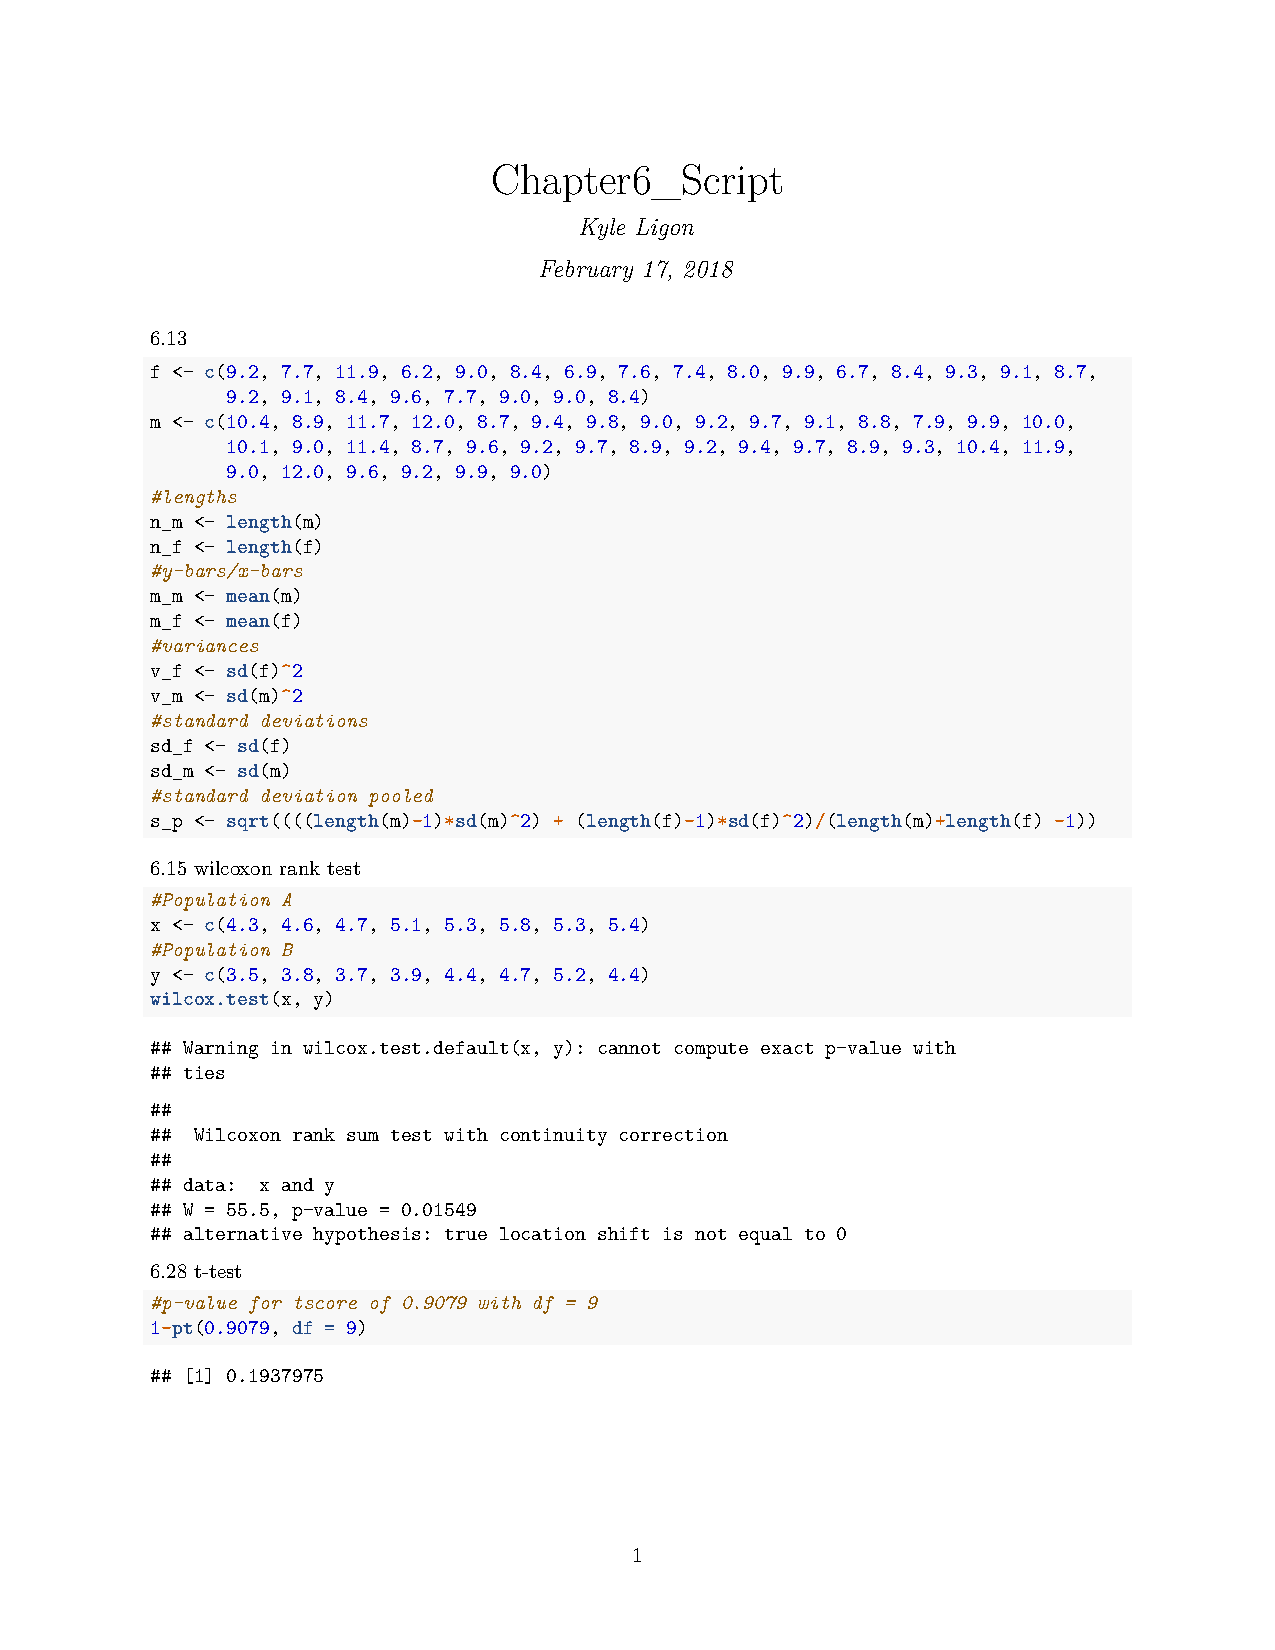
\includepdf[pages=-]{Chapter6_script.pdf}



\end{document}